\chapter{Testes e Resultados}\label{cap:conclusão}
Neste capítulo são detalhados os testes de desenvolvimento e performance do aplicativo jogo e uma descrição e resultados dos testes práticos com crianças.

\section{Testes de Desenvolvimento}


\subsection{\textbf{Teste de Tempo de Resposta do Reconhecimento}}

Após o término do desenvolvimento do protótipo, foram realizados testes para mensurar o tempo médio de resposta do algoritmo de reconhecimento por quantidade de bloco. A metodologia adotada para esse teste foi capturar uma amostra de imagens com blocos normais, imagens contendo 1 bloco, 2 blocos e com 3 blocos e uma amostra de imagens com com blocos numéricos, também com imagens contendo 1 bloco, 2 blocos e 3 blocos como ilustrado na Figura \ref{figura:ttr}. Por meio dessas imagens, foram realizadas 5 medições do tempo de resposta do algoritmo de reconhecimento por quantidade de blocos, isto é, 5 medições das imagens com apenas 1 bloco, 5 medições das imagens com 2 blocos e por fim 3 medições das imagens com 3 blocos. Após todos os valores coletados, foi calculado uma média simples por quantidade de blocos e por tipos de blocos a fim de diminuir possíveis eventualidades que afetassem o tempo de resposta. O objetivo deste teste é verificar se há diferença no tempo de resposta entre blocos normais e blocos numéricos, os quais passam pela etapa de reconhecimento óptico de caracteres.

\begin{figure}[H]
    \caption{Exemplos de Imagens para Teste de Tempo de Resposta}
    \centering
    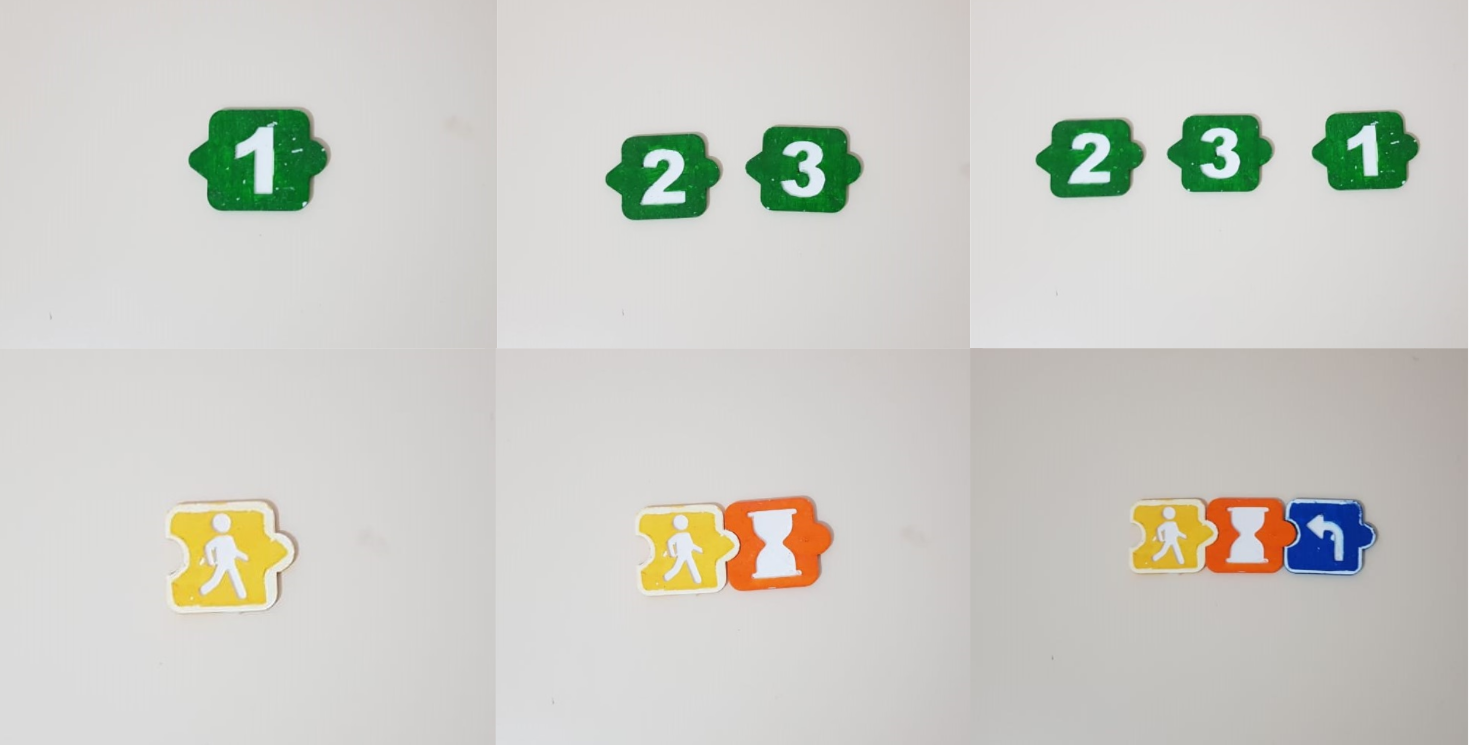
\includegraphics[width=15cm]{Imagens/Cap5/ttr.png}
    \legend{\small{Fonte: os autores (2020)}}
    \label{figura:ttr}
\end{figure}

Como pode-se ver na tabela \ref{table:tempo_resposta} e no gráfico ilustrado na Figura \ref{figura:ttr_grafico} que derivam do resultado do teste de tempos de resposta, existe uma diferença considerável no tempo de resposta entre blocos normais e blocos numéricos e essa diferença tende a crescer considerando o acréscimo de blocos. Pode-se notar também que o tempo de resposta dos blocos normais tende a se manter estável mesmo com a inserção de mais blocos normais. Porém, pode-se notar também que o tempo de resposta tende a aumentar consideravelmente com o acréscimo de blocos numéricos. 

    \begin{table}[H]
        \centering
        \caption{Tempo(s) de resposta por quantidade e tipo de bloco }
        \label{table:tempo_resposta}
        \begin{tabular}{ |c|c|c| } 
         \hline
        Quantidade de Blocos & Blocos Normais & Blocos Numéricos \\
         \hline
        1 & 0.0384s & 0.0714s \\
         \hline
        2 & 0.0434s & 0.1084s\\
         \hline
        3 & 0.0392s & 0.1503s\\    [0.5ex]    
         \hline
        
        \end{tabular}
        \legend{\small{Fonte: os autores (2020)}}
    \end{table}

\begin{figure}[H]
    \caption{Gráfico tempo de resposta}
    \centering
    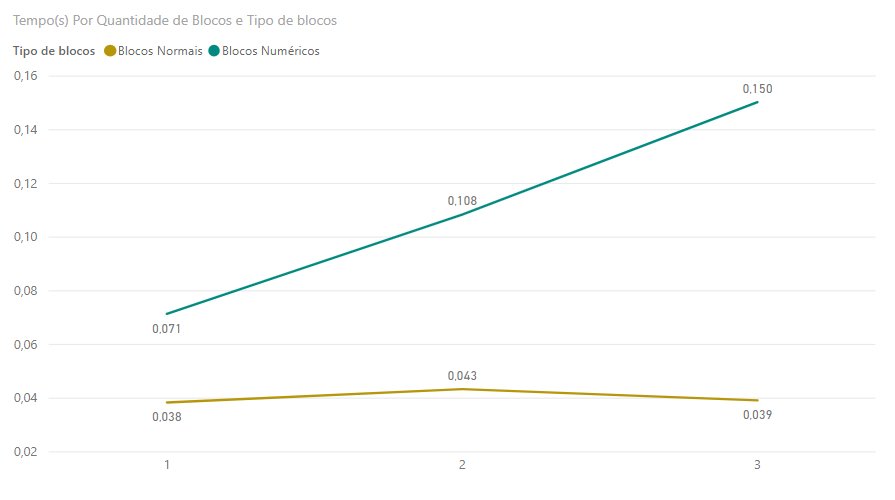
\includegraphics[width=14cm]{Imagens/Cap5/ttr_grafico.PNG}
    \legend{\small{Fonte: os autores (2020)}}
    \label{figura:ttr_grafico}
\end{figure}

\subsection{\textbf{Teste de Taxa de Assertividade do Reconhecimento}}

Após o término do desenvolvimento do protótipo, foram realizados testes para mensurar a taxa de assertividade do aplicativo jogo em relação ao reconhecimento dos blocos. A metodologia adotada para esse teste foi capturar uma amostra de imagens de uma mesma sequência de blocos, das quais uma metade dessas imagens são capturadas com iluminação adequada e seguindo as recomendações do aplicativo jogo, e a outra metade das imagens capturadas com iluminação inadequada e sem seguir as recomendações de captura do aplicativo jogo. E por meio dessas imagens, calcular as taxas de acerto para os dois tipos de imagens com o objetivo de verificar e mensurar a importância de usar o aplicativo jogo em um ambiente iluminado adequadamente e seguindo as recomendações do aplicativo jogo em relação a captura das imagens. Uma imagem considerada iluminada adequadamente é uma imagem que está sob  iluminação semelhante a iluminação utilizada para fazer a calibração do algoritmo de reconhecimento, e recomenda-se que a calibração seja realizada em um ambiente iluminado uniformemente com luz branca. 

Para o teste de assertividade, foi coletado uma amostra de 20 imagens com a sequência andar, andar, esperar, virar e andar. Das 20 imagens, 10 imagens foram coletadas sob iluminação semelhante a utilizada na calibração do algoritmo e seguindo a orientação de tamanho sugerida na tela de captura de imagem do aplicativo jogo, como ilustrado na Figura \ref{figura:tta_boa}. As outras 10 imagens, da mesma sequência, foram coletadas sob iluminação diferente da utilizada para calibração, com distâncias diferentes das recomendadas pelo aplicativo jogo e sob trepidações no momento da captura, ou seja, imagens borradas, como ilustrado na Figura \ref{figura:tta_ruim}.

\begin{figure}[H]
    \caption{Imagens adequadas para teste de assertividade}
    \centering
    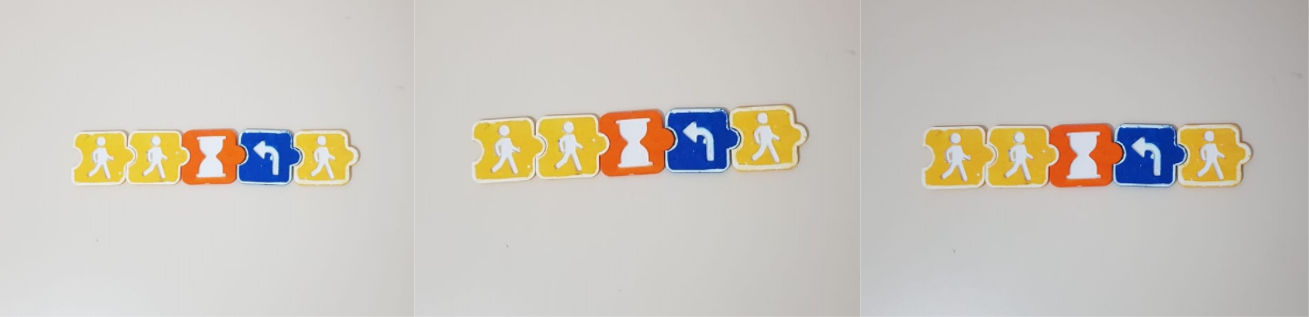
\includegraphics[width=15cm]{Imagens/Cap5/tta_boa.PNG}
    \legend{\small{Fonte: os autores (2020)}}
    \label{figura:tta_boa}
\end{figure}

\begin{figure}[H]
    \caption{Imagens não adequadas para teste de assertividade}
    \centering
    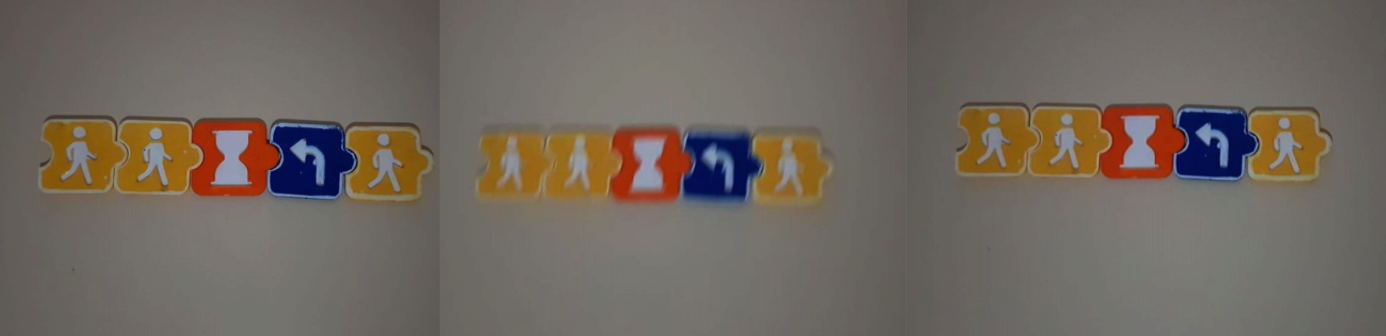
\includegraphics[width=15cm]{Imagens/Cap5/tta_ruim.PNG}
    \legend{\small{Fonte: os autores (2020)}}
    \label{figura:tta_ruim}
\end{figure}

O resultado do teste foi, das 10 imagens iluminadas adequadamente e capturadas sob as recomendações do aplicativo jogo, o algoritmo de reconhecimento acertou 9 das sequências dessas imagens, portanto obteve uma taxa de assertividade de 90 porcento. Porém, das 10 imagens iluminadas inadequadamente e que não foram capturadas seguindo as recomendações do aplicativo, o algoritmo acertou apenas 5 sequências das 10 imagens, ou seja, obteve uma taxa de assertividade de 50 porcento. Portanto, pode-se concluir que é fundamental que o aplicativo jogo seja utilizado em um ambiente adequadamente iluminado e seguindo as recomendações de captura de imagem a fim de garantir um bom funcionamento do aplicativo jogo.


\section{Testes Práticos}

\subsection{\textbf{Descrição}}


A metodologia de teste com crianças proposta pelos pesquisadores foi submetida e obteve a aprovação do comitê de ética. Portanto, antes de iniciar as etapas descritas abaixo, foi apresentado aos participantes os objetivos e a metodologia da pesquisa. A participação foi  realizada apenas após a assinatura do Termo de Consentimento Livre e Esclarecido (TCLE) pelos responsáveis. Os participante também receberam uma via do TCLE assinado pelo pesquisador responsável. Os dados pessoais coletados, como nome e idade, serão acessados apenas pela equipe de pesquisa. Todos os dados serão destruídos, no prazo de, no máximo, 1 ano.

Pensando nas eventualidades causadas pelo vírus Sars-CoV-2, causador da pandemia mundial do covid-19 no ano de 2020, os testes descritos abaixo foram realizados integralmente seguindo as orientações da OMS \cite{oms_2020} de prevenção ao Sars-CoV-2.

Os testes práticos foram realizados em duas etapas. A primeira etapa foi a resolução dos desafios propostos pelo jogo e a segunda etapa foi a resposta ao questionário de pesquisa criado pelos pesquisadores. A primeira etapa foi realizada pela criança e a segunda etapa pode ser realizada pela criança com, ou sem, o auxílio de um responsável que tenha acompanhado a aplicação da primeira etapa. Os testes foram realizados com X participantes.

Na primeira etapa os participantes jogaram o jogo dentro do ambiente de sua escolha. Os pesquisadores foram até o local de aplicação para disponibilizar os blocos físicos, celular com o aplicativo e explicar o
funcionamento do jogo para os responsáveis e as crianças. A aplicação da primeira foi será supervisionada pelos responsáveis e pesquisadores. Os participante jogaram o  aplicativo jogo por um tempo entre 15 a 30 minutos.

Na segunda etapa da pesquisa, o participante respondeu  a um questionário online que foi disponibilizado após o término da primeira etapa e ficou disponível por uma semana. O objetivo foi  validar a efetividade do aplicativo jogo em relação ao engajamento do participante, competência em ensinar programação e
capacidade de ensinar sobre reciclagem. Foi disponibilizado ao participante ou responsável, por meio do Whatsapp ou e-mail, o link do questionário. O questionário possui 5 perguntas obrigatórias e estima-se que o tempo de preenchimento do questionário seja de aproximadamente 15 minutos. As perguntas são: 1 - Qual seu primeiro nome ?; 2 - Qual a sua idade ? 3 - Você se sentiu motivado a continuar jogando o jogo ? Na pergunta 4 e 5, foram mostradas ao respondente, a imagem de um labirinto Figura \ref{figura:q4}, semelhante ao do jogo, e uma imagem de uma garrafa plástica Figura \ref{figura:q5} respectivamente, todas com 4 alternativas , das quais apenas uma é correta. 4 - Qual sequência corresponde a resolução do labirinto abaixo? a) \uparrow,  \leftarrow, \uparrow, \rightarrow$ ; b) $\uparrow, \leftarrow, \leftarrow, \uparrow, \rightarrow, \rightarrow, \rightarrow, \rightarrow$; c) $\uparrow, \leftarrow, \leftarrow, \uparrow, \rightarrow, \rightarrow, \rightarrow$; d) $\leftarrow, \leftarrow, \uparrow, \rightarrow, \rightarrow, \rightarrow, \rightarrow$ ; 5 - Em qual das lixeiras você descartaria o lixo abaixo? a) Imagem de uma lixeira azul; b) Imagem de uma lixeira amarela; c) Imagem de uma lixeira vermelha; d) Imagem de uma lixeira verde.

\begin{figure}[H]
    \caption{Pergunta 4}
    \centering
    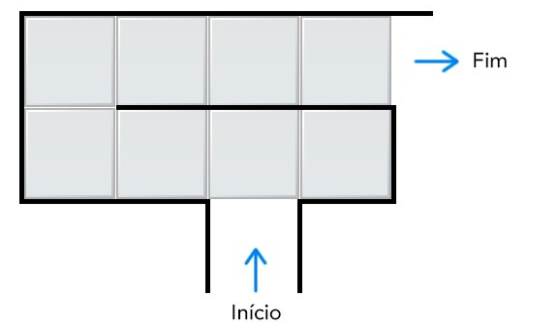
\includegraphics[width=10cm]{Imagens/Cap5/Q4.png}
    \legend{\small{Fonte: os autores (2020)}}
    \label{figura:q4}
\end{figure}


\begin{figure}[H]
    \caption{Pergunta 5}
    \centering
    
\includegraphics[width=10cm]{Imagens/Cap5/Q5.png}
    \legend{\small{Fonte: os autores (2020)}}
    \label{figura:q5}
\end{figure}

\subsection{\textbf{Teste com Crianças}}


\section{Conclusão}


Neste trabalho foi estudado a falta de recursos tecnológicos de baixo custo e fácil utilização para educação básica. Além disso, pensando nas profissões do futuro, foi visto a importância do ensino de lógica de programação para as crianças de hoje (2020).
Pensando nesses problemas apresentados, foi proposto e desenvolvido um aplicativo que tem o objetivo de tentar ensinar programação para crianças do ensino básico e fundamental 1. O aplicativo é um jogo que interage com blocos físicos por meio de reconhecimento de imagem. O aplicativo consiste em um jogo com o tema de reciclagem no qual por meio de blocos físicos, com instruções de andar, virar, esperar, repetir e blocos numerados de 0 a 9, a criança deve resolver desafios de lógica proposto pelo jogo organizando esses blocos em sequências lógicas, fotografando e submento pelo aplicativo para validar se suas instruções estão corretas ou não. O aplicativo foi desenvolvido em Unity e Python3 e os blocos foram impressos por uma impressora 3D e coloridos manualmente com tinta. O resultado final do aplicativo atendeu à todos os requisitos que foram propostos no Capítulo \ref{cap:intro} deste trabalho.

Após o término do desenvolvimento do aplicativo jogo, foram realizados teste com crianças. O objetivo destes testes foram analisar a capacidade do aplicativo jogo em reter a atenção da crianças, capacidade de ensinar conceitos básicos de programação e competência de ensinar sobre reciclagem.


Durante o desenvolvimento do aplicativo jogo, foi identificado identificado algumas possibilidades de otimização para este trabalho, como por exemplo a escolha das cores dos blocos. Por meio dos testes práticos, foi observado que a cor amarelo não se comporta bem na etapa de reconhecimento de imagem pois quando é exposta diretamente a luz tem seus parâmetros de RGB facilmente distorcidos.


\clearpage

\section{Trabalhos Futuros}

Após a conclusão do trabalho, foi identificado também possibilidade de continuações para trabalhos futuros. Como possíveis trabalhos futuros, pode-se apontar:

\begin{enumerate}
    \item Desenvolvimento do aplicativo para outros sistemas operacionais, como o iOS. 
    
    \item Desenvolvimento de novos tipos de blocos.
    
    \item Desenvolvimento de novas fases que utilizem mais blocos ou até mesmo outros tipos de blocos.
    
    \item  Refinar o algoritmo de reconhecimento dos blocos para reconhecer blocos desenvolvidos com outros materiais, desta forma, seria possível disponibilizar um pdf com instruções de montagem de blocos e desta forma a própria criança, por meio desse passo a passo, poderia construir seus blocos com papel, deixando assim a solução ainda mais econômica.

    
\end{enumerate}









